先行研究( TODO: ref)では,モデルに依存するパラメータを調節するために,
計算モデルが記述されたMODファイルからnmodlを介して生成されたCファイルを手動で変更を加えることで最適化を図っていた.\\
本研究では,自動チューニングを目的としているため,このプロセスも自動化する必要があり,そのためにこのMODからCへ変換するトランスパイラを作成した.\\
MODをパースするにあたってはDomain-Specific Languagesを作成するためのPythonライブラリである,textX ( TODO: ref)を利用し,
またMODのContext Free GrammarはMODファイルからNeuroMLを生成するためのプロジェクトであるpynmodl ( TODO: ref)のプログラムを用いた.\\

\subsubsection{nmodl}
NEURONに付属しているトランスパイラであるnmodlは,MODファイルをlexとyacc ( TODO: lex yaccの参照)を用いてパースした情報を
C言語のテンプレートに埋め込むことで対応するC言語のファイルを出力している.\\
このテンプレート化された部分の中にはNEURON本体とリンクさせるために必要な情報も多数あるため,
本研究で作成するトランスパイラもnmodlのC言語テンプレートをベースに利用した.\\

\subsubsection{実装}
( TODO: 章番号)のアルゴリズムで触れた中で,トランスパイラ内で実装を行ったのはモデルに依存するパラメータであり,
NEURON本体で細胞単位での計算の並列化等の設定もできるため,主に逐次プログラムの最適化を主眼に置いた.\\

MODファイルをC言語のファイルに変換する際,変換されたC言語のファイルは\\
・nmodl内でテンプレート化されている共通部分\\
・グローバル変数や関数定義部分\\
・ユーザー定義関数部分\\
・NEURON本体と関連する関数部分\\
・ODE(微分方程式)を計算する関数部分\\
・それぞれの関数や変数をNEURONとリンクさせる部分
の6つに分けることができる.\\
これらの関数は最後のリンクさせる部分を除き独立性が高いため,図\ref{fig:transpiler}のように,
textXを用いて作成した抽象木から最適化に用いる情報を取り出したのち,それぞれの部分を個別に最適化し
ベースとなるテンプレートにJinja2というPythonのテンプレートエンジンライブラリを用いて埋め込む形で実装を行った.\\
\begin{figure}[htb]
% h:here, t:top, b:bottom, p:page
  \begin{center}
    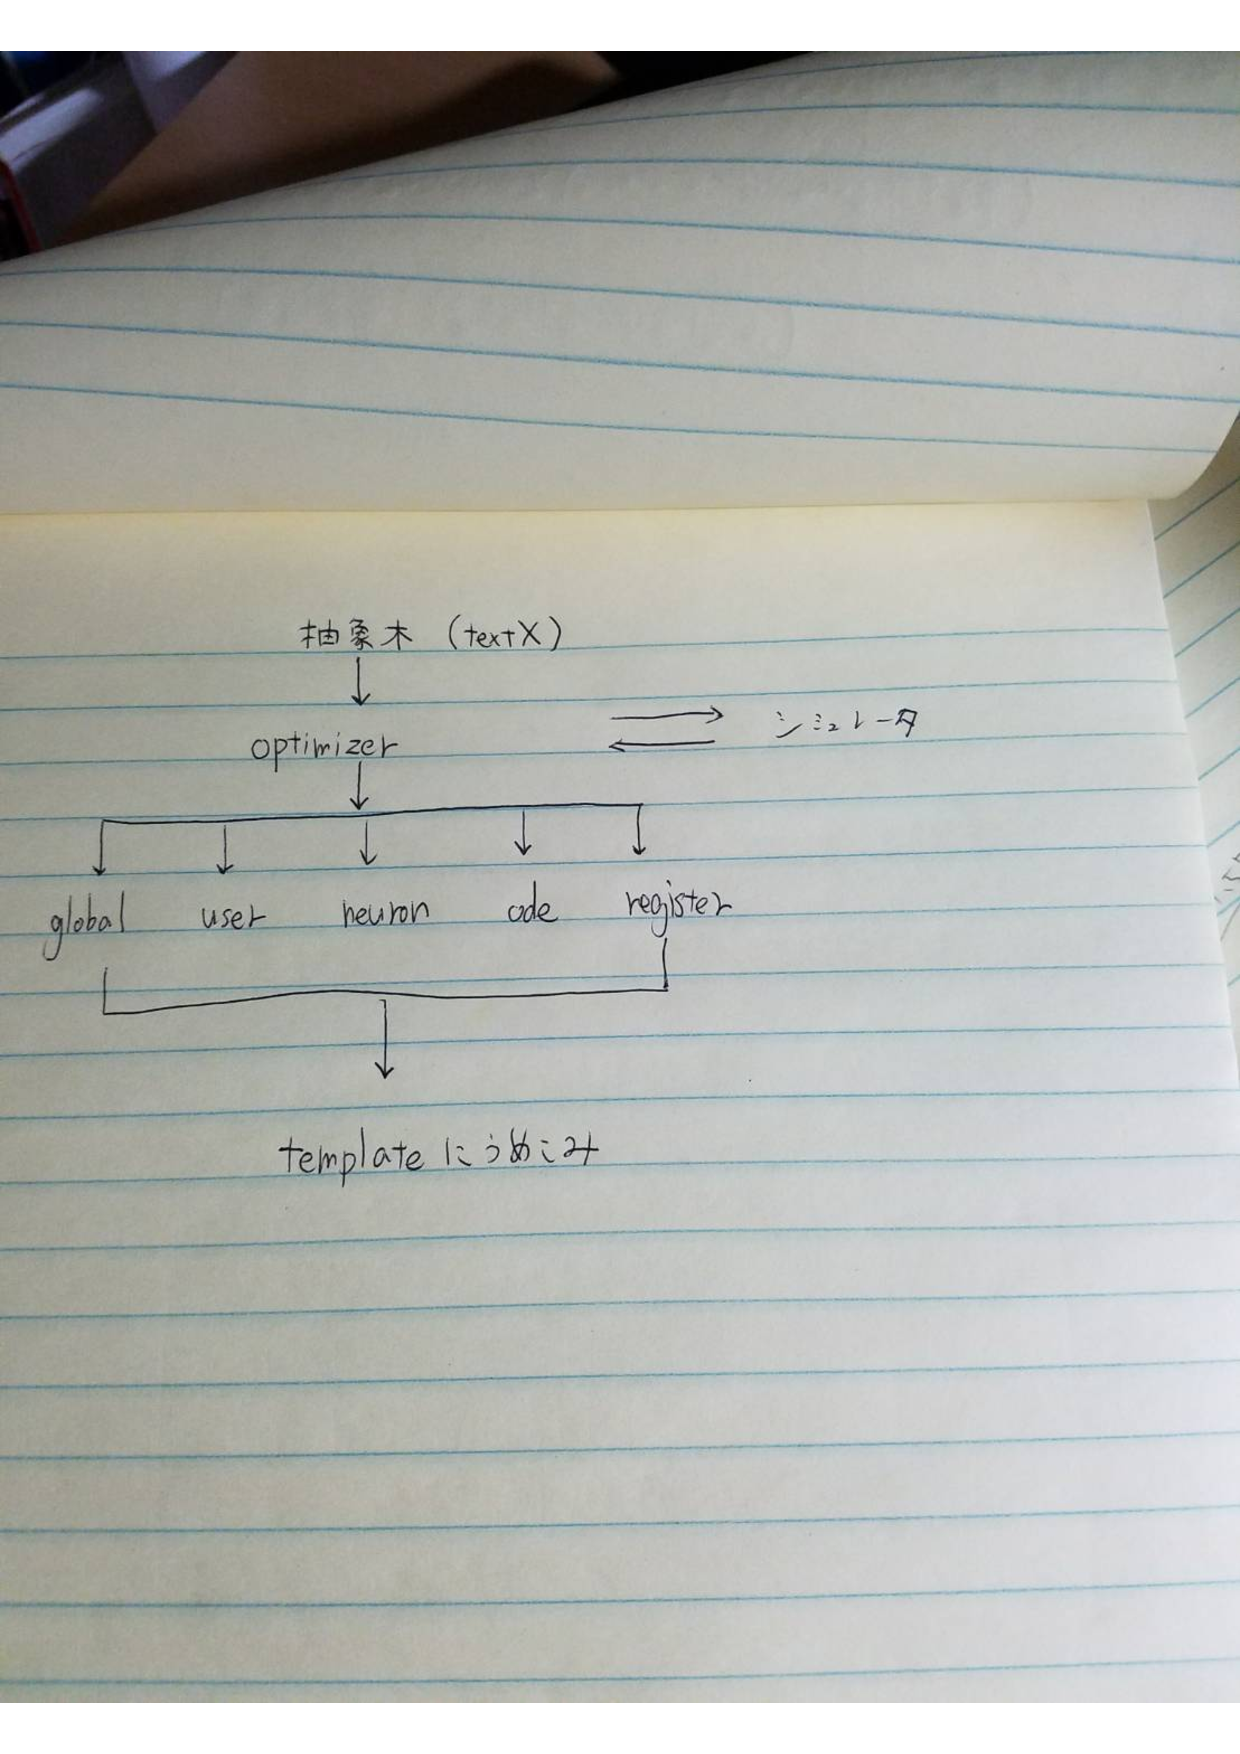
\includegraphics[width=10.0cm]{./images/transpiler.pdf}
    \caption{トランスパイラ 構成}
    \label{fig:transpiler}
  \end{center}
\end{figure}~\\
またこの構成にすることで,それぞれのモジュールごとに担当する部位が小さく細かい最適化ができるだけでなく
シミュレータ側でoptimizerからの情報を元にどの最適化を行うかを指定することができる.\\
さらに,コードを生成する部分と抽象木を作成する部分そして最適化情報を解析する部分を分離することで,
それぞれの独立性が高くなり,後から最適化の手法を追加することも容易になっている.\\

\paragraph{SIMD化}~\\
SIMD化を行うに当たって,MODファイルの中で利用されている変数を取り出す必要がある.\\
これは前述のhh.modを例にすると\\

の部分から取得できることがわかる.\\
pynmodlの中ではDerivativeと名前がつけられているため,\\

とすることで,一覧を取得することができる.\\
またこうして取得した変数名を実際のC言語のコードに変換する際に関与するのは定義部分のグローバル変数の定義部分と
各関数内での呼び出しであるが,これらに関してはすべてマクロを定義することで配列構造に変わっていたとしても同様の
アクセスができるように構成した.\\

\paragraph{配列構造のくくり出し}~\\
アルゴリズムの章において,Union-Find木を用いてMODファイル内の式を分類することでくくり出せる変数をグルーピングする手法について述べた.\\
ここではシミュレータにトランスパイラを組み込んで実行する際の実装について示す.\\
